\section{Deployment Scenarios}
\label{sec:deployments}

%%% DEPLOYMENT SCENARIOS DIAGRAM.
\begin{figure*}[ht]
  \centering
  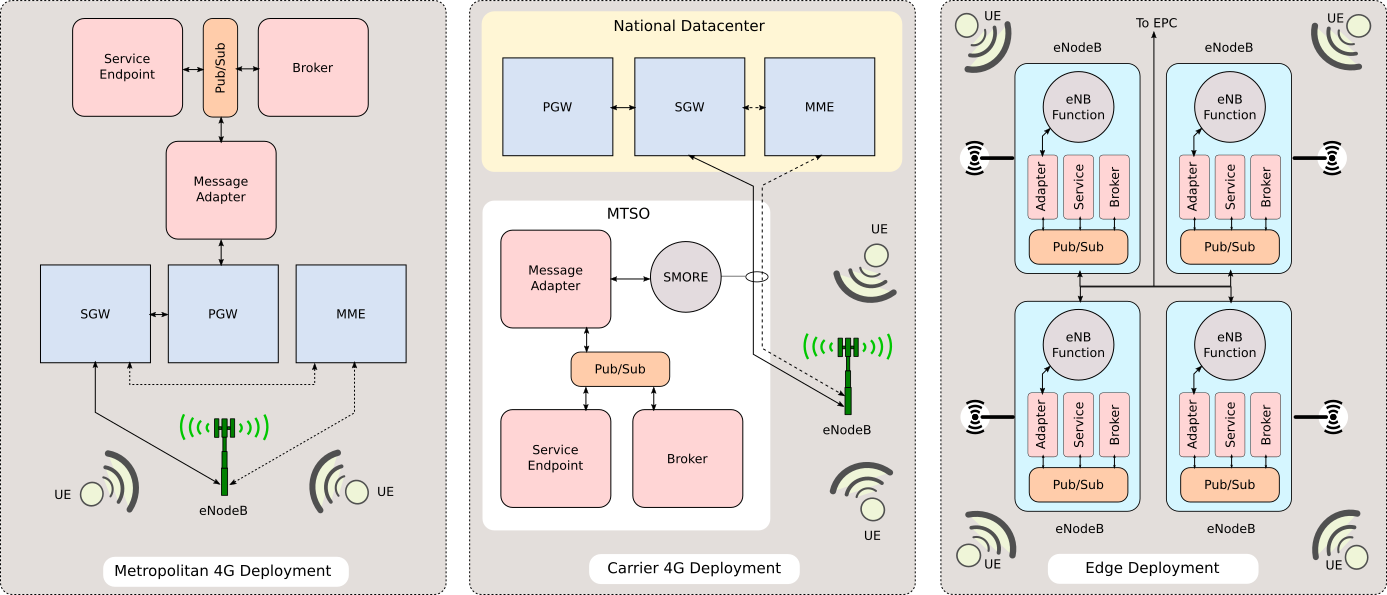
\includegraphics[width=\textwidth]{figs/deploy.png}
  \caption{\name{} deployment scenarios.}
  \label{fig:deployments}
\end{figure*}

A key aspect of the \name{} design is adaptability to different mobile
network deployments and architectures. Endpoints, broker, and pubsub
components are all mobile-environment agnostic. Mobile endpoint
identity is specific to the \name{} messaging system. One of the message
adapter's primary functions is to separate the concerns of the
messaging system with the routing of messages inside the mobile
network.  \name{} requires a low-latency vantage point near the mobile
network edge. Message adapters, pubsub, and broker all need to reside
at this vantage point.  Such proximity allows for message delivery to
meet timing requirements.  Distance to endpoints incurs a tradeoff between
convenience of deployment and ability to meet timing needs. We show
deployment versus distance/latency requirements in
table~\ref{tab:lat-req}.


\begin{table}[h]
  \centering
  \begin{tabular}{| l | l | l |}
    \hline
    \textbf{Latency Tolerance} & \textbf{Examples} & \textbf{Ref} \\ \hline \hline
    High ($> 1$ second) & Consumer info, Congestion & \cite{camp2005vehicle,papadimitratos2009vehicular} \\ \hline
    Medium ($< 50$ msec) & Lane change assistance & \cite{FIXME} \\ \hline
    Low ($< 10$ msec) & Vehicle control loop & \cite{hansson2002integrating} \\ \hline
    \hline
  \end{tabular}
  \label{tab:lat-req}
  \caption{Latenct tolerances for different types of vehicular environment messages.}
\end{table}

The message adapter can utilize different techniques to interface with
a mobile network deployment. In the simplest case, it can interact
with endpoints via routed network addresses (e.g. IPv4 or
IPv6). Alternatively, it may transparently interpose on encapsulated
communication channels to inject/extract messages (e.g. GTP
bearers). Another option is for the message adapter to operate in
concert with the wireless access point right at the edge. It could do
this by transparently interposing on the access point's data plane
uplink, or via an integrated side channel added into the access point
software.  We next present three plausible deployment scenarios, each
of which is shown in figure~\ref{fig:deployments}.

\subsection{Metropolitan area 4G deployment}
\label{sec:metro-deploy}

Consider a city investing in Intelligent Transportation System
infrastructure. Resources include a data center within the city and
wireless coverage via eNodeBs (particularly along major vehicle
corridors). The 4G EPC components reside in the local data center,
including the PGW.  Given a maximum cabling distance from the data
center to any eNodeB of around 100~kilometers, one way speed of light
latency is bounded to less than 5~milliseconds.  LTE one-way wireless
first-hop target latency is 5~ms, but may be more like
10~ms~\cite{laner2012comparison} due to UE and eNodeB processing overhead.
Further switch/router hops within the data center should not
appreciably add to the latency. Egress through SGW/PGW can add another
5~ms of one-way delay.  Total mobile network
infrastructure RTT is thus bounded to 40~ms. This leaves 10~ms for
\name{} components to process messages for low-latency
vehicle-to-vehicle coordination (within 50 ms).

In this deployment, the \name{} message adapter, pubsub, and broker
all reside alongside the PGW in the local metro data center. The
message adapter and mobile endpoints communicate using native network
addresses (i.e. IPv4 or IPv6).  \name{} components communicate via the
data center pubsub deployment. The endpoints can obtain the address
of their associated message adapter using DNS, DHCP options, or
multicast query.

\subsection{Existing mobile carrier 4G network deployment}

In an existing 4G mobile carrier network, there may not be a
centralized upstream network egress location in a particular metro
area of interest. Further, PGW nodes are typically deployed at a
handful of national data centers.  Total one-way latency to egress
through a PGW in such deployments is often over
50~ms~\cite[Chapter~7]{grigorik2013high}. Installing \name{} at these national
data centers would impair its ability to meet SLAs for some classes of
low-latency messages (see table~\ref{tab:lat-req}). Many mobile
carriers, however, concentrate regional connectivity at a Mobile
Telephone Switching Office (MTSO).  Typical one-way latency from
eNodeB to MTSO is 10~ms~\cite{cho2014smore}. With LTE RAN latency
added, the one way latency between MTSO and UE is about 20~ms.

Deployed into a MTSO, \name{} message adapters can interpose on GTP
data bearers for UEs in the same way that SMORE~\cite{cho2014smore}
does. Alternatively, lower-capacity (thus cheaper) combined SGW/PGW
functions may be deployed into the MTSO. This would allow the provider
to setup dedicated bearers for services such as \name{} in a MTSO
location.  Using these options, \name{} can operate with slightly
higher RTT compared to metropolitan data center deployments.  However,
the additional latency may not meet the latency requirements for some
UE-to-UE (vehicle-to-vehicle) applications.

\subsection{Mobile edge 4G/5G deployments}

\name{} can be altered to run at the network edge, on the mobile
wireless access points.  If a deployment includes the ability for
running services on the eNodeB (or equivalent) access points, then
\name{} can operate using peer-to-peer semantics.  All components of
\name{} would run on each eNodeB, and some service endpoints as
well. The pubsub is extended to form a connectivity mesh between
adjacent eNodeBs. \name's scope at each eNodeB is smaller, and so
the amount of processing is reduced. When a message destination is an
area of interest, the local \name{} broker determines whether parts of
this area lie outside of its coverage.  If so, it sends such messages
along (via pubsub mesh) to neighboring eNodeBs. These handle their
portion of the endpoints in the AOI.  Arbitrary consumer content
messages are also sent along to potential subscribers via the pubsub
mesh.  This deployment scenario allows for very low-latency messaging
between nodes connected via the same eNodeB (potentially under 20~ms
RTT considering RAN latency). Inter-eNodeB communication latency
depends on the communication path between eNodeBs.  This could be only
a handful of milliseconds if there are metro-area-local paths.

A second realization of this deployment scenario is via a 5G CloudRAN
environment~\cite{checko2015cloud}. Here eNodeBs are split into remote radio
heads (RRH) connected to base band units (BBUs).  The latter are
located in nearby compute aggregation locations; RRH and BBU functions
can only be about 25~km apart in order to maintain the closed control
loop between them. BBU functionality in a compute location serves
multiple RRH units. \name{} components would be deployed into the
compute locations in this case.  Multiple such compute locations may
serve an area. \name{} could be deployed to each with a peer-to-peer
pubsub mesh setup between them.  Similar very low latency messaging is
possible in this scenario with a \name{} message adapter working with
the BBUs at its location.  An additional advantage is that the very
low latency messaging extends to the (larger) area covered by all
associated RRH units.
